\documentclass[10pt]{article}
\usepackage[polish]{babel}
\usepackage[utf8]{inputenc}
\usepackage[T1]{fontenc}
\usepackage{amsmath}
\usepackage{amsfonts}
\usepackage{amssymb}
\usepackage[version=4]{mhchem}
\usepackage{stmaryrd}
\usepackage{graphicx}
\usepackage[export]{adjustbox}
\graphicspath{ {./images/} }

\title{LIGA MATEMATYCZNA \\
 im. Zdzisława Matuskiego GRUDZIEŃ 2022 \\
 SZKOŁA PODSTAWOWA \\
 klasy IV - VI }

\author{}
\date{}


\begin{document}
\maketitle
\section*{ZADANIE 1.}
Znajdź takie trzy cyfry, z których można utworzyć dwa różne trzycyfrowe sześciany liczb naturalnych. Podaj sumę znalezionych cyfr.

\section*{ZADANIE 2.}
Różnica cyfr liczby dwucyfrowej jest równa 5 . Różnica tej liczby i liczby utworzonej z niej przez przestawienie cyfr jest równa 45. Znajdź te liczby.

\section*{ZADANIE 3.}
Do przygotowania paczek świątecznych Mikołaj użył 120 mandarynek i 180 pierników. W każdej paczce jest jednakowa liczba mandarynek i jednakowa liczba pierników. Ile maksymalnie paczek udało się przygotować?

\section*{ZADANIE 4.}
Pan Kowalski ma pięciu synów: Adama, Bartka, Czarka, Darka i Edka. Przygotował dla nich pod choinkę pię́c prezentów: album ze zdjęciami wozów policyjnych, piłkę, wóz strażacki, klocki i misia. Każdy z chłopców otrzymał jeden prezent. Wiadomo, że

\begin{itemize}
  \item najstarszy syn dostał album, a najmłodszy misia;
  \item Czarek jest starszy od Bartka, ale młodszy od Edka i nie dostał klocków;
  \item Adam ma czterech starszych braci;
  \item Bartek dostał piłkę;
  \item Darek nie jest najstarszy.
\end{itemize}

Jaki prezent dostał każdy z chłopców?

\section*{ZADANIE 5.}
Mikołaj położył dziewięć orzechów na planszy \(9 \times 9\) w sposób przedstawiony na rysunku. Po chwili Ania przełożyła trzy orzechy na sąsiednie pola (to znaczy na pola mające wspólny wierzchołek lub bok), a sześć zostało na swoich miejscach. Mimo że trzy orzechy zmieniły miejsce, to nadal w każdym rzędzie poziomym i pionowym znajduje się jeden orzech. Pokaż w jaki sposób Ania przełożyła orzechy.\\
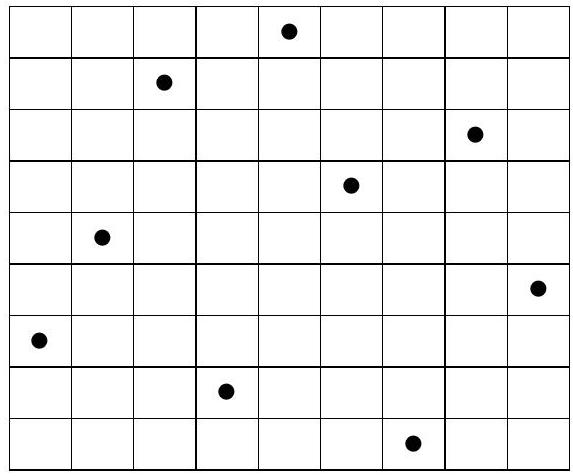
\includegraphics[max width=\textwidth, center]{2024_11_21_1d80345ac4b2b7e80bbfg-1}


\end{document}